\section{Entwurf des Data Warehouse}
\subsection{Relationale Umsetzung eines MDM-Schemas}
Zur Realisierung, der in Phase 1 entworfenen Data Cubes, sollen die nachfolgenden relationalen Modelle verwendet werden. Es wurde sich hierbei für das Starflake-Schema entschieden, da es die Vorteile des Star- und Snowflake-Schemas vereint. Die notwendigen Befehle zum Anlegen der Dimensions- und Faktentabelle sind in der beigefügten SQL-Datei zu finden. 

\subsubsection{Data Cube für die Anzahl der Bestellungen}
\begin{figure}[htbp] 
    \centering
       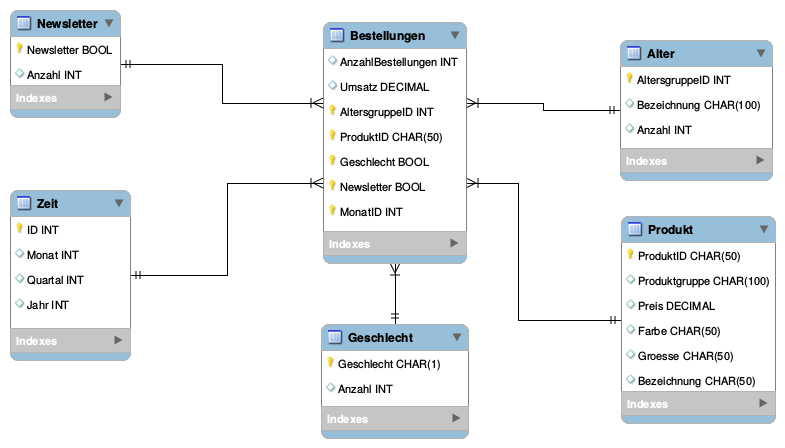
\includegraphics[width=0.8\textwidth]{phase2/dwh-bestellungen.png}
    \caption{Relationales Umsetzung des Cubes \glqq Bestellungen\grqq}
    \label{fig:bestellungen}
  \end{figure} 
   
Der Data Cube \glqq Bestellungen\grqq ~setzt sich aus der Faktentabelle \glqq Bestellungen\grqq ~und den Dimensiontabellen \glqq Alter\grqq ,~\glqq Produkt\grqq ~und \glqq Geschlecht\grqq ~zusammen. Die Dimension \glqq Zeit\grqq ~wurde gemäß dem Snowflake-Ansatz für eine bessere Datenintegrität in die Relationen \glqq Monat\grqq , \glqq Quartal\grqq ~und \glqq Jahr\grqq ~unterteilt.
\pagebreak

\subsubsection{Data Cube für die Anzahl der Retouren}
\begin{figure}[htbp] 
    \centering
       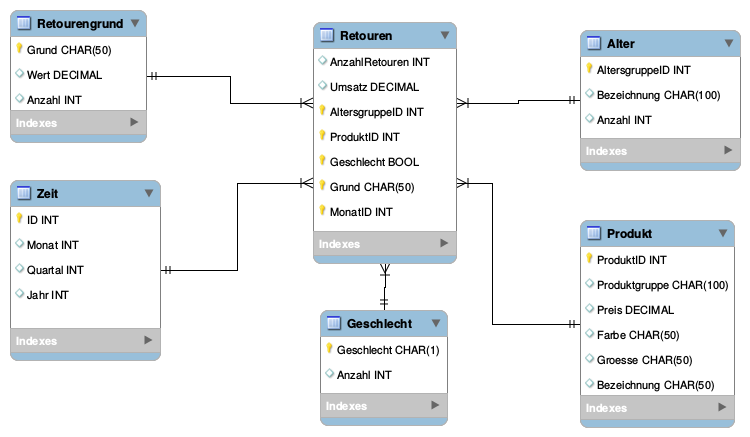
\includegraphics[width=0.8\textwidth]{phase2/dwh-retouren.png}
    \caption{Relationales Umsetzung des Cubes \glqq Retouren\grqq}
    \label{fig:retouren}
\end{figure}  
Analog zum Cube \glqq Bestellungen\grqq ~wurde auch der Data Cube \glqq Retouren\grqq ~zur Analyse der Reklamationen in eine Faktentabelle und mehrere Dimensionstabellen untergliedert. Auch hier wurde sich zur Verbesserung der Datenintegrität dazu entschieden, die Dimension \glqq Zeit\grqq ~in mehrere Tabellen aufzuteilen 
  
  
\subsubsection{Data Cube für Cross-Sells}
\begin{figure}[htbp] 
    \centering
       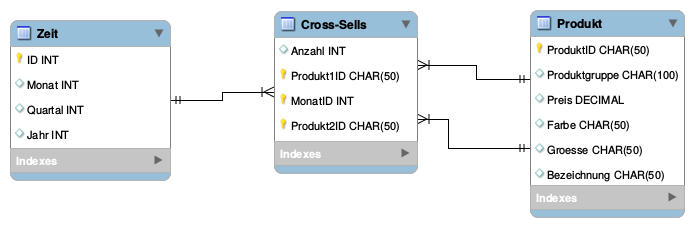
\includegraphics[width=0.72\textwidth]{phase2/dwh-cross.png}
    \caption{Relationales Umsetzung des Cubes \glqq Cross-Sells\grqq}
    \label{fig:bestellungen}
  \end{figure}  
  
Mithilfe des Data Cubes \glqq Cross-Sells\grqq ~soll, wie bereits erwähnt, untersucht werden, welche Produkte besonders häufig zusammen gekauft werden. Da zwischen den Produkten eine Art m-zu-n-Beziehung besteht, besitzt die Faktentabelle \glqq Cross-Sells\grqq ~zwei Fremdschlüssel auf die Dimensionstabelle \glqq Produkt\grqq . Auch bei diesem Cube wurde sich dazu entschieden, die zeitliche Dimension aufzuspalten.
  
\subsection{Optimierung der Data Cubes}
Zur Optimierung der Data Cubes stehen verschiedene Möglichkeiten zur Verfügung. So könnten durch materialisierte Sichten sowohl für die Cubes also auch für die Basis-Datenbank das Laden der Daten bzw. der Analyseprozess beschleunigt werden. Dabei wäre es ausreichend, wenn diese wöchentlich aktualisiert werden. Auch die Verwendung von Indexen wäre denkbar, um so die Abarbeitung bestimmter Analyseabfragen zu beschleunigen.